\section{Packet transactions}
\label{s:transactions}

\begin{figure*}[!t]
\begin{subfigure}{0.5\textwidth}
\begin{small}
\begin{lstlisting}[style=customc]
#define NUM_FLOWLETS    8000
#define THRESHOLD       5
#define NUM_HOPS        10

struct Packet {
  int sport;
  int dport;
  int new_hop;
  int arrival;
  int next_hop;
  int id; // array index
};

int last_time [NUM_FLOWLETS] = {0};
int saved_hop [NUM_FLOWLETS] = {0};

void flowlet(struct Packet pkt) {
  pkt.new_hop = hash3(pkt.sport,
                      pkt.dport,
                      pkt.arrival)
                % NUM_HOPS;

  pkt.id  = hash2(pkt.sport,
                  pkt.dport)
            % NUM_FLOWLETS;

  if (pkt.arrival - last_time[pkt.id] @\label{line:ifStart}@
      > THRESHOLD)
  { saved_hop[pkt.id] = pkt.new_hop; } @\label{line:ifEnd}@

  last_time[pkt.id] = pkt.arrival;
  pkt.next_hop = saved_hop[pkt.id];
}
\end{lstlisting}
\end{small}
\caption{Flowlet switching written in \pktlanguage}
\label{fig:flowlet_code}
\end{subfigure}
%
%
\begin{subfigure}{0.4\textwidth}
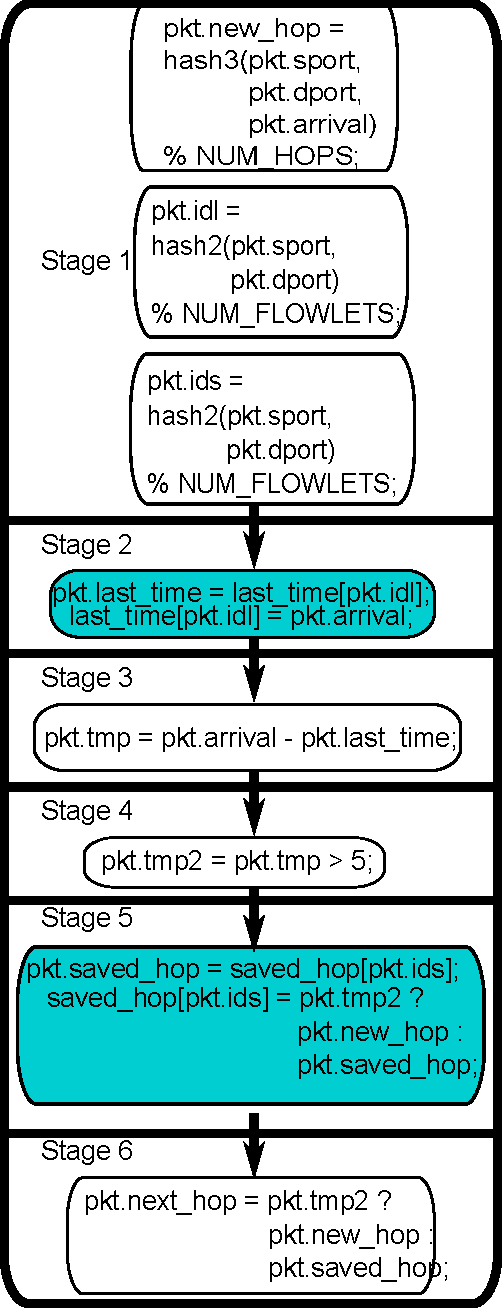
\includegraphics[width=0.9\columnwidth]{pipe.pdf}
\caption{6-stage \absmachine pipeline for flowlet
switching.  Control flows from top to bottom. Stateful atoms are in grey.}
\label{fig:flowlet_pipeline}
\end{subfigure}
\caption{Programming flowlet switching in \pktlanguage}
\end{figure*}

To program a data-plane algorithm, a programmer would write code in
\pktlanguage using packet transactions (Figure~\ref{fig:flowlet_code}).  The
\pktlanguage compiler then compiles this transaction to an atom pipeline for a
\absmachine machine (Figure~\ref{fig:flowlet_pipeline}). We first describe
packet transactions in greater detail by walking through an example
(\S\ref{ss:flowlet}). Next, we discuss constraints in \pktlanguage
(\S\ref{ss:constraints}) informed by line-rate switches.  We then discuss
triggering packet transactions (\S\ref{ss:guards}) and handling multiple
transactions (\S\ref{ss:multiple}).

\subsection{\pktlanguage by example}
\label{ss:flowlet}

We use flowlet switching~\cite{flowlets} as our running example. Flowlet
switching is a load-balancing algorithm that sends bursts of packets (called
flowlets) from a TCP flow on a randomly chosen next hop, provided the bursts
are separated by a large enough time interval to ensure packets do not arrive
out of order at a TCP receiver. For ease of exposition, we use only the source
and destination ports in the hash function that randomly computes the next hop
for flowlet switching.
%it is easy to extend it to the full 5-tuple.

Figure~\ref{fig:flowlet_code} shows flowlet switching in \pktlanguage and
demonstrates its core language constructs. All packet processing happens in the
context of a packet transaction (the function \texttt{flowlet} starting at line
17). The function's argument type {\tt Packet} declares the fields in a packet
(lines 5--12)\footnote{We use fields to refer to both packet headers such as
source port ({\tt sport}) and destination port ({\tt dport}) and packet
metadata ({\tt id}).} that can be referenced by the function body (lines
18--32).  The function body can also modify persistent switch state using
global variables (e.g.  \texttt{last\_time} and \texttt{saved\_hop} on lines 14
and 15, respectively). The function body may use \textit{intrinsics} such as
\texttt{hash2} on line 23 to directly access hardware accelerators on the
switch such as hash generators.  The \pktlanguage compiler uses an intrinsic's
signature when analyzing dependencies, but otherwise treats it as a blackbox.
%TODO: Rethink intrinsic description

\paragraph{Packet transaction semantics}
Semantically, the programmer sees the switch invoking the packet transaction
serially in the order in which packets arrive, with no concurrent packet
processing.  Put differently, the packet transaction modifies the passed-in
packet argument and runs to completion, before starting on the next packet.
Practically, the switch exploits parallelism within and across pipeline
stages to sustain line rate. The \pktlanguage compiler bridges
these two views: it converts the packet transaction in
Figure~\ref{fig:flowlet_code} to the atom pipeline in
Figure~\ref{fig:flowlet_pipeline}, and guarantees the semantics of a packet
transaction.
% TODO: This could come all the way at the beginning of this section.

\subsection{Constraints on the language}
\label{ss:constraints}
\pktlanguage's syntax (Figure~\ref{fig:grammar}) is similar to C, but with
several constraints (Table~\ref{tab:restrict}).  These constraints are required
for deterministic performance.  Memory allocation, unbounded iteration counts,
and unstructured control flow cause variable performance, which may prevent an
algorithm from achieving line rate.  Additionally, \pktlanguage constrains
array modifications by requiring that all accesses to a given array within one
execution of a transaction, i.e., one packet, must use the same array index.
For example, all read and write accesses to the array \texttt{last\_time} use
the index \texttt{pkt.id}, which is constant for each packet, but can change
between packets. This restriction mirrors restrictions on the stateful memories
attached to atoms (\S\ref{s:atomConstraints}), which require multiple ports to
support distinct read and write addresses every clock cycle.

\begin{table}
  \begin{tabular}{p{0.9\columnwidth}}
    No iteration (while, for, do-while).\\
    No goto, break, or continue.\\
    No pointers.\\
    No dynamic memory allocation / heap.\\
    Array index is constant for each transaction execution.\\
    No access to the unparsed portion of the packet.\\
%    No arrays in packet fields.\\
  \end{tabular}
  \caption{Restrictions in \pktlanguage}
  \label{tab:restrict}
\end{table}

\begin{figure}
\newcommand{\sep}{~|~}
\begin{scriptsize}
\begin{eqnarray*}
e \in expr &::=& e.f \sep c \sep var \sep e_1~op~e_2 \sep \neg~e \sep e[e] \sep f(\ldots) \\
%
s \in stmt &::=& e = e \sep if~(c)~s_1~else~s_2 \sep s~;~s \\
%
t \in pktTxn &::=& txnName(Packet) \{ s \} \\
%
d \in pktDecl &::=& Packet \{ v~;~v \} \\
%TODO, Doesn't there need to be a * or + here (one or more variables in a packet field)?.
%TODO: Also are all restrictions supposed to be captured in the grammar?
%
sv \in stateVarDecl &::=& v = e \sep sv \\
%
p \in program &::=& \{ d ; sv ; t \}
\end{eqnarray*}
\end{scriptsize}
\caption{\pktlanguage grammar}
\label{fig:grammar}
\end{figure}

\subsection{Triggering packet transactions}
\label{ss:guards}
Packet transactions specify \textit{how} to process packet headers and/or
state.  To specify {\em when} to run packet transactions, we provide a {\em
guard}: a predicate on packet fields that triggers the transaction whenever a
packet matches the guard. An example guard (pkt.tcp\_dst\_port == 80) would
trigger heavy-hitter detection on all packets on TCP destination port 80. This
guard can be realized using an exact match in a match-action table, with the
actions being the atoms compiled from a packet transaction. Guards
can take various forms, e.g., exact, ternary, longest-prefix, and range-based
matches, depending on the matches supported by the match-action
pipeline. Because guards map rather straightforwardly to the match key in a
match-action table, we focus only on compiling packet transactions.

% Anirudh->Alvin: Guards are outside the Domino language. They are whatever
% match semantics is supported by the switch.
% This is a practical requirement to express data-plane algorithms on a real switch, but not something very interesting to talk about.

\subsection{Handling multiple transactions}
\label{ss:multiple}
So far, we have discussed a single packet transaction corresponding to a single
data-plane algorithm. In practice, a switch would run multiple data-plane
algorithms, each processing its own subset of packets. To address this, we
envision a policy language that specifies pairs of guards and transactions.
Realizing a policy is straightforward when all guards are disjoint. When guards
overlap, multiple transactions need to execute on the same subset of packets,
requiring a mechanism to compose transactions. One semantics for composition is
to concatenate the two transaction bodies in an order specified by the user,
providing the illusion of a larger transaction that combines two transactions.
We leave a detailed exploration of this and alternative semantics to future
work, and focus only on compiling a single packet transaction.

%%\ac{would interleaving stmts from multiple transactions be a potential
%%optimization here (as in db transactions)?}
%% Possibly: I don't quite know how to reason about the semantics yet :) We should talk about this, sometime!

%%\ac{is the user going to 
%%provide how transactions will be concatenated?}
%% Yes, the user specifies the order of concatenation. The how is basically paste one trans. body, and then the other, and call it a larger transaction.
